% pf.tex — Perfect hash function diagram
\documentclass[border=2pt]{standalone}

\usepackage{tikz}
\usepackage{amsmath,amssymb}
\usetikzlibrary{arrows.meta,positioning,calc}

\begin{document}
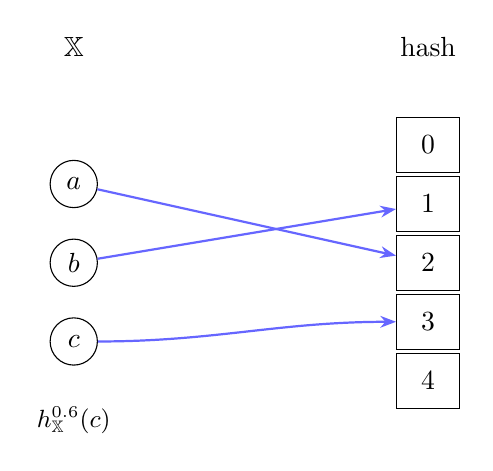
\begin{tikzpicture}[
  key/.style={circle,draw,fill=white,minimum size=6mm,inner sep=1pt},
  slot/.style={rectangle,draw,minimum width=8mm,minimum height=7mm,inner sep=2pt},
  arrow/.style={-{Stealth[length=2mm]},thick}
]

% Input set label
\node[above] at (1,4.5) {$\mathbb{X}$};

% Input keys (left side)
\node[key] (a) at (1,3) {$a$};
\node[key] (b) at (1,2) {$b$};
\node[key] (c) at (1,1) {$c$};

% Hash table label
\node[above] at (5.5,4.5) {hash};

% Hash table (right side) - 5 slots numbered 0-4
\node[slot] (h0) at (5.5,3.5) {$0$};
\node[slot] (h1) at (5.5,2.75) {$1$};
\node[slot] (h2) at (5.5,2) {$2$};
\node[slot] (h3) at (5.5,1.25) {$3$};
\node[slot] (h4) at (5.5,0.5) {$4$};

% Arrows showing perfect hash mapping
\draw[arrow,blue!60] (a) -- (h2);
\draw[arrow,blue!60] (b) -- (h1);
\draw[arrow,blue!60] (c) to[out=0,in=180] (h3);

% Label for one of the hash computations
\node[below,font=\small] at (c |- 0,0.3) {$h_{\mathbb{X}}^{0.6}(c)$};

\end{tikzpicture}
\end{document}
